\section{External effects and the ambiguous timeout}\label{sec:C13:effects}
The difficult interruption occurs between an external effect and recording its receipt. Suppose an agent submits a transaction, the remote service commits it, and the network response is lost. The local system observes a timeout. Retrying can duplicate the effect; assuming success can advance a task whose operation actually failed. A session transcript containing ``tool timed out'' does not distinguish these worlds. This is an information problem before it is a language-model problem.

Represent an effect by an operation identifier $k$, a payload digest $d$, a target resource, and a state from a declared effect state machine. A useful application-level sequence is proposed, authorized, dispatched, confirmed, and reconciled. ``Unknown'' is a legitimate state after a timeout. It should not be silently mapped to failure. If the remote service supports a stable idempotency key and records the corresponding result, retries with the same key can retrieve or complete the same logical operation under that service's contract. Without such support, exactly-once external execution cannot be inferred from local retries.

The ambiguity admits a minimal impossibility witness. Let $w_0$ be a world in which the first attempt did not commit and $w_1$ one in which it committed but its receipt was lost. Assume that both produce the same local observation and that an unkeyed retry commits once in either world. Let $D$ indicate a duplicate effect and $O$ an omitted required effect. If the recovery policy retries with probability $r$, then
\begin{align}
 P(D=1\mid w_1)&=r,\\
 P(O=1\mid w_0)&=1-r,\\
 \max\{r,1-r\}&\geq\tfrac12.
\end{align}
Omission here means failing to realize the required effect under a policy that terminates after this recovery choice. No policy based solely on the indistinguishable local record can guarantee both completion and absence of duplication. Indefinite abstention avoids a new effect but does not establish completion. A status query, a service-enforced operation key, or additional external evidence changes the information structure and can break the witness. This is an analytical construction, not an observed failure rate; its bound must not be applied to services whose retry contract differs.

The following proposed state transition separates validation, durable intent, external dispatch, and evidence-based reconciliation. Let $u$ be a command instance including its logical intent identity, $J$ its local journal, and $\alpha$ current authority. The predicate $v(u,\alpha)\in\{0,1\}$ checks schema and access to the corresponding journal scope. For $v(u,\alpha)=1$, let $k=\eta(u)$ identify this logical operation, $p(u)$ its payload, and $d=h(p(u))$ the payload digest. The stable identifier is reused on recovery; equal payloads alone do not identify the same user intent. Define $\gamma(u,J,\alpha)=1$ exactly when $v(u,\alpha)=1$ and either $k$ is absent from $J$ or its record binds the same logical intent identity and exact payload as $u$; otherwise $\gamma(u,J,\alpha)=0$. A digest match alone does not establish that binding. Let $\sigma_J(k)\in\{\varnothing,\iota,\upsilon,\kappa_+,\kappa_-\}$ denote absence, persisted intent with no acknowledged dispatch marker, marked possible dispatch with unresolved outcome, confirmed effect, and confirmed absence of the specified effect. All callers must obey the marker-before-call ordering; otherwise an intent-only record does not establish absence of dispatch. For an absent or intent-only operation admitted by $\gamma=1$, the fresh-dispatch branch $\Phi_0$ is
\begin{equation}
\begin{aligned}
 J_1&=\mathcal I(J;k,d,u,\alpha),\\
 J_D&=\mathcal M(J_1;k),\\
 r&\sim\mathcal D(\,\cdot\mid k,u),\qquad J_D\ne\bot_J,\quad a_D(u,\alpha)=1,\\
 J_2&=
 \begin{cases}
  \mathcal P(J_D;k,r),&\chi(r)\ne\bot,\\
  \mathcal U(J_D;k),&\chi(r)=\bot,
 \end{cases}\\
 \Phi_0(u,J,\alpha)&=\sigma_{J_2}(k).
\end{aligned}
\label{eq:C13:intent_dispatch_receipt}
\end{equation}
Here $\mathcal I$ durably records the intent and $\mathcal M$ durably marks possible dispatch, changing $\iota$ to $\upsilon$ before the call. The local branch selection and marker transition assume a serialized dispatcher for each key or an equivalent atomic, fenced claim; separate lookup and unconditional writes do not enforce that assumption. The separate predicate $a_D(u,\alpha)$ checks current authority for new dispatch, including service-side concurrency conditions. If it is false, $\Phi_0=\bot_A$ and none of the displayed fresh-dispatch operations is evaluated. Reading a terminal receipt is governed by journal access and need not require the old write permission. The receipt classifier $\chi(r)\in\{1,0,\bot\}$ denotes confirmed effect, confirmed absence of the specified effect, or unresolved status. The operator $\mathcal P$ persists either confirmed class; $\mathcal U$ records uncertainty. A transport acknowledgment alone is not effect confirmation. Every journal operator returns an acknowledged journal or $\bot_J$; the next line is evaluated only after acknowledgment. A storage failure returns $\bot_J$ and recovery begins from the last acknowledged journal. A lost receipt can therefore leave a marked, unresolved dispatch despite an external effect. A crash after the marker but before the call is also unresolved: this conservative false ambiguity prevents an unsafe automatic retry.

Let $e$ be evidence acquired through a separately authorized reconciliation path; unavailable or inconclusive evidence leaves $\upsilon$ unchanged. With $\mathcal R$ restricted to evidence updates and never issuing the original effect, define
\begin{equation}
\begin{aligned}
 \Phi_R(u,J,\alpha;e)&=\sigma_{\mathcal R(J;k,e)}(k),\\
 \Phi(u,J,\alpha;e)&=
 \begin{cases}
  \bot,&\gamma(u,J,\alpha)=0,\\
  \sigma_J(k),&\gamma=1,\ \sigma_J(k)\in\{\kappa_+,\kappa_-\},\\
  \Phi_R(u,J,\alpha;e),&\gamma=1,\ \sigma_J(k)=\upsilon,\\
  \Phi_0(u,J,\alpha),&\gamma=1,\ \sigma_J(k)\in\{\varnothing,\iota\}.
 \end{cases}
\end{aligned}
\label{eq:C13:evidence_reconciliation}
\end{equation}
The lookup in $\Phi_R$ is evaluated only when $\mathcal R$ returns an acknowledged journal; otherwise it returns $\bot_J$. Terminal replay and unresolved reconciliation never call $\mathcal D$. In particular, current dispatch authority is necessary for a new effect but does not make an unresolved retry safe. A service-enforced retry contract can justify a different explicitly declared recovery branch; it is not assumed here. These maps specify application obligations, not an atomic transaction across the journal and remote service. Authority must be current at dispatch, even when no conversational state changed. Service-enforced key scope, retention time and payload-conflict behavior bound the idempotency guarantee; a key cached locally cannot impose that guarantee on the remote endpoint.
The reconciliation path may query the remote service, inspect a resource version, or request a human decision when the outcome cannot be determined safely. It should not ask the model to guess what probably happened. A model can assist in interpreting receipts, but the effect state must remain tied to evidence.

Linearizability supplies a precise correctness condition for concurrent objects whose operations appear to take effect at a point between invocation and response~\cite{herlihy1990linearizability}. It does not automatically extend across unrelated services or provide an application with a global transaction. A local database can atomically record an intent while an external email, payment, or deployment remains outside that transaction. Calling the local workflow durable does not make the combined operation atomic.

Compensation is another distinct mechanism. A compensating action attempts to restore an acceptable business state after an effect has happened. It need not restore the original world exactly: a sent message cannot be unsent from every recipient's memory. The agent's plan should therefore distinguish reversible local edits, remotely idempotent operations, and effects requiring compensation or manual resolution. Session recovery should preserve those distinctions through summarization.

This analysis explains why successful restart tests can be misleading. If tests interrupt only before a tool call or after its confirmed receipt, they miss the ambiguous interval. Fault injection should include the boundary after remote commit but before local acknowledgment. That experiment directly tests whether the implementation's effect model matches the guarantee claimed for long-running execution.



The loss point in Figure~\ref{fig:C13:continuity} separates remote commitment from local knowledge; a missing receipt cannot establish absence of the effect.
\begin{figure}[!htbp]
\centering
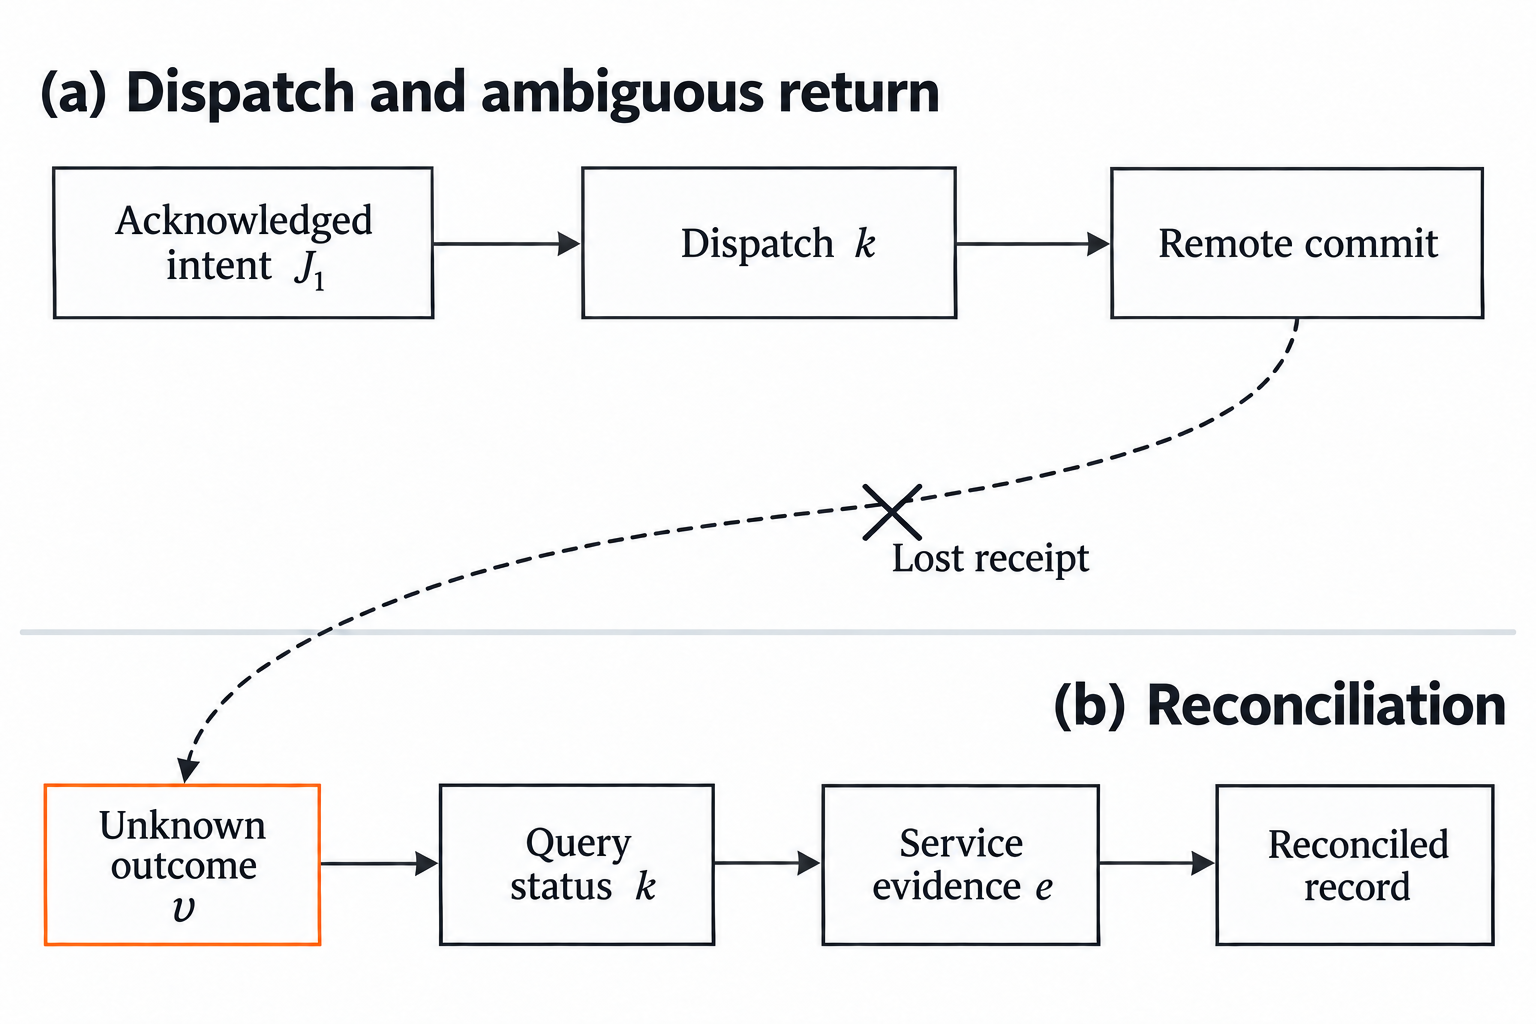
\includegraphics[width=\linewidth]{book/figures/assets/F13review.png}
\caption{An illustrative committed-but-unacknowledged operation. Confirmed intent precedes dispatch; a lost receipt after remote commit leaves the local outcome unknown. A status query obtains additional service evidence for the local record. Without conclusive evidence, that record remains unknown. The pre-call possible-dispatch mark and other admission checks are omitted. Historical replay and fresh dispatch have different authorization requirements. No global transaction or exactly-once guarantee is implied.}
\label{fig:C13:continuity}
\end{figure}
